
\documentclass[preprint,12pt]{elsarticle}

\usepackage[spanish]{babel}
\usepackage{amssymb}
\usepackage{graphicx}
\usepackage{lineno}
\usepackage[utf8]{inputenc}
\usepackage{url}
\usepackage{natbib}

\begin{document}
	
	\begin{frontmatter}

		\title{\huge  COMPARATIVA ENTRE INTELIGENCIA DE NEGOCIO (BI) Y ANALITICA DE NEGOCIO(BA) }
		\author{Robles Flores, Anthony Richard	                (2016056192)}
		\author{Estrella Palacios, Katherine Lizbeth			(2015050948)}
		\author{Sosa Bedolla, Sharon					(2016054467)}
		\author{Torres Beltran , Joihanna				(2015053235)}
		\address{Tacna, Perú}
		


%%INICIO abstract
\begin{abstract}
Contenido
\end{abstract}
%%FIN abstract


\end{frontmatter}

%%INICIO Resumen
\section{Resumen}
Contenido
%%FIN Resumen


%%INICIO Introducción
\section{Introducción}
Contenido
%%FIN Introducción



%%INICIO Marco Teórico
\section{Marco Teórico}

%%----------------------------------------------------------------------------------------------------------------------------------------------------------
	\subsection{Inteligencia de Negocios (BI)}
	Contenido\cite{referenciarobles1}



%%EJEMPLO DE COMO PONER UNA IMAGEN
\begin{figure}[htb]
\begin{center}
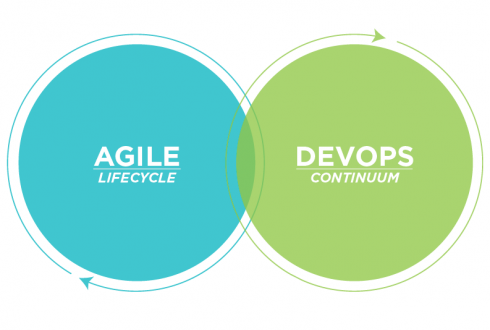
\includegraphics[width=10cm]{./IMAGENES/evolucion}
\caption{Hipervisor}
\end{center}
\end{figure}
%%


%%-----------------------------------------------------------------------------
	\subsection{Analitica de Negocio (BA) }
	CONTENIDO
	\begin{itemize}
	\item 1. 
	\item 2. 
	\item 3. 
	\end{itemize}



%%-----------------------------------------------------------------------------
	

%%----------------------------------------------------------------------------------------------------------------------------------------------------------
%%FIN Marco Teórico




%CONCLUSIONES
\section{Conclusiones}
\subsection{Conclusión }	
CONTENIDO





%RECOMENDACIONES
\section{Recomendaciones}	
CONTENIDO






	
	\newpage
	\bibliographystyle{apalike}
	\bibliography{BIBLIOGRAFIA}	
%\citep{referenciarobles2}  


\end{document}

